\chapter{WebSearch}

\section{World Wide Web}

Il Web è un'applicazione sviluppata da \textbf{Tim Berners-Lee}, nel periodo 1989-1991 per consentire alle persone di condividere infomrazioni tramite Internet.

L'architettura del web è di tipo \textbf{client-server} e il suo funzionamento può essere descritto come segue:

\begin{itemize}
    \item Le informazioni sono salvate su delle macchine \textbf{server} e resi disponibili tramite Internet sotto forma di \textbf{pagine web}.
    \item Un'applicazione \textbf{client} (browser) richiede tali pagine web pubblicamente accessibili.
\end{itemize}

A noi ciò che interessa in realtà non è \textbf{l'organizzazione fisica} ma quella \textbf{logica} delle pagine web.Le pagine web possono \textbf{referenziare} in maniera \textit{diretta} altre pagine web, tramite dei \textbf{riferimenti} o \textbf{link}. Possiamo quindi pensare al web come un grafo diretto in cui i nodi sono le pagine web, e gli archi sono i riferimenti tra una pagina e un'altra. Per questo motivo, una pagina web viene anche detta \textbf{ipertesto}.

\subsection{Precursori dell'Ipertesto}

Possiamo considerare l'ipertesto come un'implementazione del concetto di \textbf{memoria associativa}. Un primo precursore all'ipertesto è il concetto di \textbf{referecence}, ad esempio,  le citazioni all'interno di articoli o libri ad altre informazioni o autori di tali infomrazioni. Anche in questo caso si crea un grafo diretto i cui nodi sono i libri o gli articoli e gli archi sono  riferimenti.La differenza sostanziale però con l'ipertesto è la linea temporale nella quale si fanno i riferimenti. Se un libro $X$ fa una citazione a un articolo $Y$ vuol dire che $Y$ è stato scritto e pubblicato prima di $X$, perciò non ci potranno essere riferimenti ad $X$ nell'articolo $Y$.

Invece, nel grado del web capita spesso di avere archi bidirezionali, ovvero due pagine che si referenziano a vicenda.

Un altro precursore dell'ipertesto sono le cosidette \textbf{crossing-referecences}, o \textbf{riferimenti incrociati}. Tale tipo di organizzazione la troviamo per esempio in un enciclopedia, e consente di collegare argomenti differenti attraverso una catena di collegamenti semantici o riferimenti tra altri argomenti.

\begin{figure}[ht!]
    \centering
    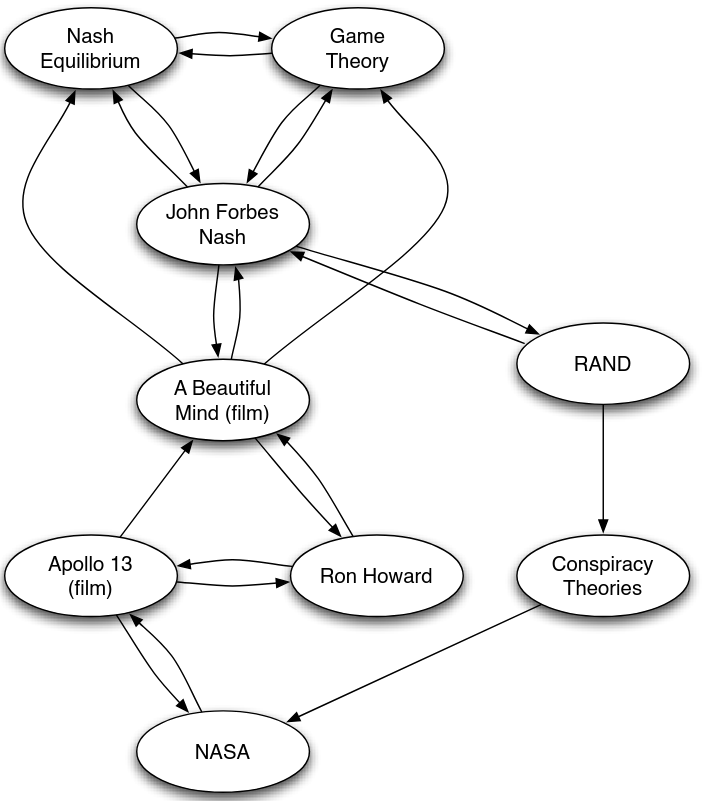
\includegraphics[width=0.5\linewidth]{images/WS_references.png}
    \caption{Esempio di crossing-referecences}
    \label{fig:WS_references}
\end{figure}

\subsection{MEMEX}

Vannevar Bush nel suo articolo "As we may think" del 1945 cercò di immaginare come le moderne tecnologie di comunizaione emergenti all'epoca avrebbero influenzato il mondo, grazie alle rivoluzionarie tecniche di \textbf{archiviazione, scambio} e \textbf{accesso} di informazioni.

In particolare Bush osservò che i metodi tradizionali per archiviare le informazioni in un libro, in una biblioteca o nella memoria di un computer erano altamente \textbf{lineari}. Basta pensare a un dizionario enciclopedico in cui tutti gli argomenti sono ordinati uno dopo l'altro.

D'altra parte la mente umana struttura e accede alla propria esperienza mostrando quella che potrebbe essere definita una \text{memoria associativa}, ovvero è strutturata in una \textbf{rete semantica} di concetti. Tu pensi a una cosa, te ne ricorda un'altra tramite una \textit{connessione}, dopodiché ti viene un intuizione che ti porta ad un terzo pensiero, e così via…

Bush ha quindi immaginato un sistema che cercava di imitare questo stile di memorizzazione \textbf{associativa}, il \textbf{MEMEX}, ovvero una versioni digitalizzate di tutta la conoscenza umana collegate da collegamenti associativi. Infatti Bush fu esplicitamente citato da Tim Berners Lee quando progettò il Web.

\subsection{Web 2.0}

Inizialmente, il web era costituito da una collezione di pagine \textbf{statiche} al cui interno erano (eventualmente) presenti degli \textit{hyperlink} ad altre pagine. Tali \textit{hyperlink} sono detti \textbf{navigazionali} in quanto servono appunto a "navigare" nel Web, esattamente come noi navighiamo nella nostra conoscenza, implmentando quindi il conetto di \textbf{memoria associativa}.

Col tempo però il web si è evoluto, passando da pagine totalmente statiche a pagine che consentono di effettuare \textbf{azioni}, come per esempio effettuare una richiesta ad un server oppure effettuare pagamenti. I link che consentono di effettuare tali azioni prendono il nome di link \textbf{transazionali}.

Altre evoluzioni sono per esempio l'avvento dei servizi, come per esempio:
\begin{itemize}
    \item La creazione e mantenimento di contenuti in maniera condivisa con Wikipedia.
    \item Lo scambio di messaggio con i servizi di web-mailing.
    \item Reti che connettono individui anziché documenti con i social-media.
    \item Reti che connettono video con YouTube.
\end{itemize}

Con tali evoluzioni si indica il cosidetto Web 2.0.

\subsection{Il Grafo Diretto del Web}

Il Web può essere visto come un grafo diretto, i cui nodi sono le \textbf{pagine} e gli archi sono gli \textbf{hyperlink} tra esse. Inoltre, è facilmente osservabile che una pagina web conosce solamente le pagine a cui stan puntando (\textbf{archi uscenti}) e non le pagine che la stanno puntando (\textbf{archi entranti}).

In uno studio del 2000, si è osservato che il grafo del web è è composto da milioni di nodi, ed ha una forma a \textbf{bowtie (a fiocco)}. Come si può osservare in \autoref{fig:WS_bowtie}, al centro è presente una \textbf{componente gigante fortemente  connessa} composta appunto dalla maggior parte dei nodi. In tale componente, per ogni pagina $X$ della componente è possibile trovare una serie link che collegano $X$ verso qualsiasi nodo della SCC, e viceversa da qualsiasi altra pagina è possibile navigare e raggiungere $X$.

\begin{figure}[ht!]
    \centering
    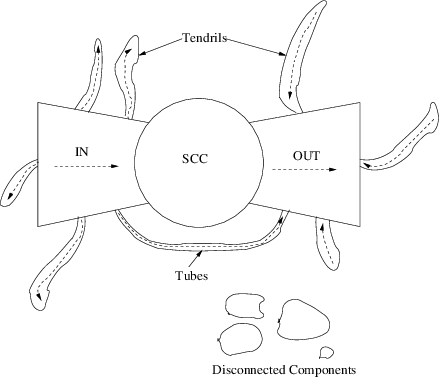
\includegraphics[width=0.5\linewidth]{images/WS_bowtie.png}
    \caption{Il grafo del web come \textbf{bowtie}}
    \label{fig:WS_bowtie}
\end{figure}

Dopodiché, si osservo la presenza di altre 2 componenti che formavano una sorta di \textit{flusso} in entrata e in uscita da SCC, le quali sono:

\begin{itemize}
    \item \textbf{IN}: composta dai nodi dai quali navigando è possibile raggiungere SCC, ma non raggiungibili in alcun modo da SCC.
    \item \textbf{OUT}: composta dai nodi raggiungibili da SCC tramite una navigazione ma che a loro volta non possono raggiungere SCC. Possiamo quindi die che questa componente rappresenta il flusso in uscita da SCC.
\end{itemize}

Infine, sono state individuate altre componenti nel grafo del web:

\begin{itemize}
    \item \textbf{Tendrilis}: detti anche \textit{tentacoli}, è una componente composta da 
    nodi che sono raggiungibili dai nodi presenti nella componente IN ma dai quali non si può raggiungere SCC e da nodi attraverso i quali si può raggiungere la componente OUT ma i quali non sono raggiungibili dai nodi in SCC.
    \item \textbf{Tubi}: composto dai nodi che creano un flusso che collega la componente IN alla componente OUT senza passare però per la componente SCC.
    \item \textbf{Componenti disconnesse}: una serie di nodi disconnessi dalla struttura a fiocco.
\end{itemize}

\section{Web Search}

Il problema di classificare e ricercare documenti è un problema antico.

Prima dell'avvento del Web, la difficoltà nel ricercare documenti era sostanzialmente dovuta alla scarsità di questi ultimi. Infatti, un tempo bisognava raggiungere fisicamente una biblioteca, libreria o archivio per avere accesso a libri, articoli o documenti, e inoltre non ce n'erano a disposizione una grande quantità. Tuttavia c'era un vantaggio, i documenti in generale erano catalogati in categorie, perciò a chi interessava avere informazioni su un determinato argomento bastava recarsi nel luogo in cui erano raccolti i documenti relativi all'argomento interessato. Per esempio, a un avvocato che necessita delle schede penali di alcune persone basta andare in un archivio di un tribunale. Oppure se ti interessa trovare un nuovo romanzo da leggere, basta andare in libreria nella sezione "Romanzi" e troverai una raccolta di libri inerenti al genere che ti interessa.

Il Web ha letteralmente capovolto i ruoli. Adesso chiunque ha acesso a una infinità di documenti in letteralmente pochissimi istanti. Il problema principale invece è appunto questa \textbf{sovrabbondanza di documenti}, i quali purtroppo non sono catalogati e raggruppati in categorie.

Purtroppo proprio per questa eterogeneità dei documenti, non è possibile effettuare una ricerca specializzata per parole chiave. Oltre al fatto che il numero di parole chiave è potenzialmente illimitato, una parola assume differenti significati. Infatti per esempio la parola "albero" in teoria dei grafi è un grafo particolare, mentre in botanica è un tipo di pianta, oppure ancora può poter significare un albero genealogico.

Si vuole quindi definire uno strumento di web search che consenta di effettuare una ricerca catalogando in base a delle parole chiave e scartando tutte le pagine non coerenti. Questa però non è una condizione sufficiente affinché uno strumento di web search risulti utile. Infatti, come risultato di una ricerca, potrebbe essere restituito un insieme potenzialmente immenso di pagine inerenti alle parole chiave. Perciò è necessario che tale strumento in qualche modo sfoltisca le pagine meno rilevanti, restituendo così un inseme abbastanza piccolo da essere umanamente visitato, e possibilmente ordinando queste pagine in un ordine di rilevanza, ovvero effettuando un \textbf{ranking} delle pagine restituite.

\subsection{Link Analisys}

Purtroppo il contenuto interno di una pagina non consente da solo di quantificarne con precisione la sua rilevanza rispetto alla ricerca in corso.

Un primo strumento utile che consente invece di capire meglio la rilevanza di una pagina sono gli \textbf{hyperlink}. 

Consideriamo prima un esempio:

Stiamo studiando un articolo utile per fare una tesi. Per capire meglio l'argomento un solo articolo non basta, perciò decidiamo di attingere alla bibliografia dell'articolo. Purtroppo notiamo che sono presenti svariate decine di citazioni ad altri articoli. Non potendo leggerli tutti quanti, è sensato considerare gli articoli che più hanno citazioni in generale.

Prendendo quindi come base questo esempio, dopo aver escluso tutte quelle pagine non inerenti alla nostra ricerca, possiamo \textbf{ordinarle} in ordine non crescente di numero di referimenti. Più precisamente, mettiamo tra i primi risultati della ricerca tutte quelle pagine che all'interno del sottoinsieme di pagine inerenti alla ricerca sono \textbf{maggiormente puntate da hyperlink}.

Ovvero la rilevanza di una pagina è calcolata analizzando i link che la coinvolgono.

\subsection{Metodo HITS}

Il primo metodo di link analisys che studiamo è il  metodo \textbf{HITS - Hyperlink-Induced Topic Search}.

Poiché consideriamo come pagine rilevanti le pagine che sono molto puntate da altre pagine nell'insieme, può accadere che una pagina è puntata da tante pagine poco rilevanti ai fini della ricerca, ad esempio, sappiamo che per finalità di marketing possono essere acquistati puntatori
ad una data pagina, così da far aumentare il suo contatore di \textbf{in-link}. Allora è necessario considerare la seguente questione:

\textit{Quando una pagina è considerata abbastanza autorevole da trasmettere rilevanza ad una pagina a cui punta?}

Il metodo HITS, associa a ciascuna pagina 2 indici:

\begin{itemize}
    \item Un indice di \textbf{autorità}: questo indice esprime la \textit{rilevanza} della pagina ai fini della ricerca.
    \item Un indice di \textbf{hub (centro, fulcro)}: questo indice esprime \textit{l'autorevolezza} della pagina a conferire autorità alle pagine alle quali punta. In altre parole indica quanto questa pagine è rilevante per la pagine a cui punta.
\end{itemize}

Intuitivamente, possiamo definire l'indice d'autorità $a_i$ della pagina $i$, come il numero di pagine attinenti alla ricerca che puntano alla pagina $i$ (\textbf{In-Degree})
\[
    a_i = |\{j: j \text{ è attinente alla ricerca e } j \rightarrow i\}|
\]

In questo modo, se consideriamo la matrice $M$ di adiancenza del sottografo del Web attinente alla ricerca, abbiamo che
\[
a_i = \sum_{j=1}^n M_{ji}
\]

Analogamente, il valore di hub $h_i$ di una pagina $i$, potrebbe essere il numero di pagine attinenti alla ricerca alle quali essa punta (\textbf{Out-Degree})

\[
    h_i = |\{j: j \text{ è attinente alla ricerca e } i \rightarrow j\}|
\]

di conseguenza, abbiamo che

\[
h_i = \sum_{j=1}^n M_{ij}
\]

dove la matrice di adiacenza $M$ del sottografo rilevante è definita come
\[
M_{ij} =
\begin{cases}
1 & \text{se } i \rightarrow j,\\[4pt]
0 & \text{altrimenti,}
\end{cases}
\qquad\text{per } i,j = 1,\dots,n.
\]


Raffiniamo il modello introducendo una dipendenza ricorsiva tra i punteggi: il punteggio di \textbf{Autorità ($a_i$)} di una pagina è proporzionale alla somma dei punteggi di \textbf{Hub} delle pagine che la puntano. Simmetricamente, il punteggio di \textbf{Hub ($h_i$)} è proporzionale alla somma dei punteggi di \textbf{Autorità} delle pagine verso cui essa punta.

\begin{itemize}
    \item Una pagina è una buona \textbf{Authority} se è linkata da ottimi \textbf{Hub}.
    \item Una pagina è un buon \textbf{Hub} se linka ottime \textbf{Authority}.
\end{itemize}

Quindi, se supponiamo di conoscere un valore iniziale di Hub, $h_i^{(0)}$ per ciascuna pagina $i$, allora

\[
a_i^{(1)} = \sum_{j=1}^n M_{ji} h_j^{(0)}
\]

e poiché il valore di autorità di ciascuna pagina è variato, potremmo calcolare il valore di hub per ottenere una valutazione migliore, ossia

\[
h_i^{(1)} = \sum_{j=1}^n M_{ij} a_j^{(1)}
\]

Quindi, al passo $k$, abbiamo che

\begin{equation}\label{eq:auth_and_hub}
\begin{split}
    a_i^{(k+1)} &= \sum_{j=1}^n M_{ji} h_j^{(k)} \\
    h_i^{(k+1)} &= \sum_{j=1}^n M_{ij} a_j^{(k+1)}
\end{split}
\end{equation}

definendo quindi un metodo iterativo per il calcolo dei valori di autorità e hub.

Poiché in genere non si hanno informazioni iniziali circa il valore del hub delle pagine che si stanno considerando, si può assumere che tali valori siano uguali per tutte le pagine, ossia
\[
\forall i = 1, \dots n,\ h_i^{(0)} = 1.
\]
Inoltre, possiamo riscrivere le equazioni \eqref{eq:auth_and_hub} nel seguente modo:

\begin{equation}
\begin{split}
    a^{(k+1)} &= M^T\ h^{(k)} \\
    h^{(k)} &= M\ a^{(k)}
\end{split}
\end{equation}

dove $a^{(k+1)}$ e $h^{(k)}$ sono vettori colonna.

Abbiamo quindi introdotto un procedimento iterativo che aggiorna progressivamente i punteggi di hub e di authority per ciascuna pagina. L'obiettivo è che, ad ogni passo, tali valori riflettano sempre meglio la rilevanza delle pagine; perché questo avvenga è però necessario che la procedura converga verso dei valori limite, che costituiscono i punteggi "reali" di hub e authority.

Le relazioni che aggiornano i vettori $a^{(k)}$ e $h^{(k)}$ sono somme di termini non negativi; di conseguenza i loro valori tendono ad aumentare con le iterazioni e non convergono verso un vettore limite. Perciò la convergenza ha senso solo dopo l'applicazione di un'opportuna \textbf{normalizzazione}.

\begin{teorema}\label{teo:th_hits}
    Esistono un valore \(c\in\mathbb{R}_{>0}\) e un vettore \(z\in\mathbb{R}^n\), \(z\neq 0\), tali che per ogni vettore iniziale \(h^{(0)}\) con coordinate strettamente positive si ha
    \[
        \lim_{k\to\infty}\frac{h^{(k)}}{c^k}=z
        \qquad\text{e}\qquad
        \lim_{k\to\infty}\frac{a^{(k)}}{c^k}=z.
    \]
\end{teorema}

\newpage

\subsubsection{Richiami di Algebra Lineare}

Prima di dimostrare questo teorema è necessario ricordare alcune nozioni di algebra lineare.

\begin{definizione}[Autovalore e Autovettore]
    Data una matrice quadrata $A \in \mathbb{R}^{n\times n}$, un vettore $x \in \mathbb{C}^n$ e un valore $\lambda \in \mathbb{C},\ \lambda \neq 0$, diremo che $x$ e $\lambda$ sono rispettivamente un \textbf{autovettore} e un \textbf{autovalore} per $A$ se e solo se
    \[
        Ax = \lambda x
    \]
\end{definizione}

\begin{teorema}\label{teo:th_rosso}
    Sia \(A\in\mathbb{R}^{n\times n}\) simmetrica. Allora tutti gli autovalori di \(A\) sono reali (contati con la molteplicità) ed esiste una base ortonormale di \(\mathbb{R}^n\) formata da autovettori di \(A\).
\end{teorema}

\begin{definizione}[Base]
    Un insieme di vettori $\{z_1,\dots,z_n\}\subset\mathbb{R}^n$ si dice \textbf{base} di $\mathbb{R}^n$ se soddisfa una (e quindi entrambe) delle seguenti proprietà equivalenti:
    \begin{enumerate}
        \item ogni vettore $x\in\mathbb{R}^n$ si può esprimere come combinazione lineare dei $z_i$, ovvero esistono scalari $c_1,\dots,c_n\in\mathbb{R}$ tali che
        \[
            x=\sum_{i=1}^n c_i z_i;
        \]
        \item i vettori $z_1,\dots,z_n$ sono linearmente indipendenti.
    \end{enumerate}
    Inoltre, in questo caso la scrittura di $x$ come combinazione lineare dei $z_i$ è unica.
\end{definizione}

\begin{definizione}[Ortonormale]
    Sia $\{z_1,\dots,z_n\} \subset \mathbb{R}^n$, con $z_i=(z_{i1},\dots,z_{in})$.
    Diciamo che la famiglia è \emph{ortonormale} se per ogni \(i=1,\dots,n\) vale \(\|z_i\|=1\) e per ogni \(i\neq j\) si ha \(\langle z_i,z_j\rangle=0\).
\end{definizione}

\begin{definizione}[Matrice semidefinita positiva]
    Una matrice simmetrica \(A\in\mathbb{R}^{n\times n}\) si dice \emph{semidefinita positiva} se
    \[
        \forall x\in\mathbb{R}^n:\quad x^{T} A x \ge 0.
    \]
\end{definizione}

\begin{teorema}\label{teo:th_blu}
    Sia $A\in\mathbb{R}^{n\times n}$ una matrice semidefinita positiva. Allora:
    \begin{enumerate}
        \item tutti gli autovalori di $A$ sono maggiori o uguali a $0$;
        \item se $A\neq 0$, allora esiste almeno un autovalore strettamente positivo.
    \end{enumerate}
\end{teorema}

\newpage

\subsubsection{Dimostrazione del Teorema}

Dimostriamo ora il \autoref{teo:th_hits} usando i due teoremi appena enunciati, \autoref{teo:th_rosso} e \autoref{teo:th_blu}.

\begin{proof}[\autoref{teo:th_hits}]
    Per iniziare la dimostrazione, richiamiamo le espressioni per gli indici di autorità e hub:
    \[
    \begin{aligned}
        a^{(k+1)} &= M^T h^{(k)},\\
        h^{(k)}   &= M a^{(k)}.
    \end{aligned}
    \]

    \begin{description}
        \item[Osservazione 1.] La matrice $M M^T$ è reale e simmetrica:
        \[
        (M M^T)_{ij}=\sum_{k=1}^{n}M_{ik}(M^T)_{kj}=\sum_{k=1}^{n}M_{ik}M_{jk}=(M M^T)_{ji}.
        \]
        Per il \autoref{teo:th_rosso}, $M M^T$ ammette una base ortonormale di autovettori e tutti i suoi autovalori sono reali.
        \item[Osservazione 2.] $M M^T$ è semidefinita positiva: per ogni $x\in\mathbb{R}^n$
        \[
        x^T(M M^T)x=(x^T M)(M^T x)=\|M^T x\|^2\ge 0.
        \]
        infatti, ponendo
        \begin{align*}
            &y = (M^T x) = (y_1, y_2, \dots, y_n) \\
            &y^T = (x^T M) = (y_1, y_2, \dots, y_n)^T
        \end{align*}
        si ottiene
        \[
        x^T(M M^T)x = (x^T M)(M^T x) = y^T\ y = \sum_{k=1}^{n} y^2_{k} \ge 0
        \]
        Essendo $M M^T\neq 0$, dal \autoref{teo:th_blu} segue che il suo autovalore massimo è strettamente positivo.
    \end{description}

    Usando le relazioni ricorsive otteniamo:
    \[
    \begin{aligned}
        h^{(1)} &= M a^{(1)} = M M^T h^{(0)},\\
        h^{(2)} &= M a^{(2)} = (M M^T) h^{(1)} = (M M^T)^2 h^{(0)},\\
        &\ \vdots\\
        h^{(k)} &= (M M^T)^k h^{(0)}.
    \end{aligned}
    \]

    Sia ora $\{z_1,\dots,z_n\}$ una \textbf{base ortonormale} di autovettori reali di $MM^T$, con autovalori non negativi corrispondenti $c_1,\dots,c_n$ tali che
    \[
    (MM^T) z_i = c_i z_i,\qquad i=1,\dots,n.
    \]
    Senza perdita di generalità ordiniamo gli autovalori in modo decrescente:
    \[
    c_1 \ge c_2 \ge \dots \ge c_n,
    \]
    ricordando che $c_1>0$.
    Possiamo quindi esprimere $h^{(0)}$ come combinazione lineare degli autovettori:
    \[
    h^{(0)} = \sum_{i=1}^{n} q_iz_i \text{ scelti opportuni scalari } q_i 
    \]

    Di conseguenza, 
    \begin{align*}
        h^{(k)} &= (M M^T)^k h^{(0)} = (M M^T)^k \sum_{i=1}^{n} q_iz_i \\
        &= (M M^T)^{k-1} \sum_{i=1}^{n} q_i (M M^T) z_i = (M M^T)^{k-1} \sum_{i=1}^{n} q_i c_i z_i \text{ per definizione di autovalore} \\
        &= (M M^T)^{k-2} \sum_{i=1}^{n} q_i c_i (M M^T) z_i = (M M^T)^{k-2} \sum_{i=1}^{n} q_i c_i^2 z_i \\
        &\vdots \\
        h^{(k)} &= \sum_{i=1}^{n} q_i c_i^k z_i
    \end{align*}

    Dividiamo ora entrambi i membri per $c_1^k$ e otteniamo
    \[
    \frac{h^{(k)}}{c_1^k} = \sum_{i=1}^{n} q_i \left(\frac{c_i}{c_1} \right)^k z_i
    \]

    Poiché l'autovalore massimo può presentarsi con molteplicità maggiore di uno, indichiamo con \(l\) (con \(1\le l\le n\)) il numero di autovalori pari a tale valore massimo, ossia
    \[
    c_1 = c_2 = \dots = c_l > c_{l+1} \ge \dots \ge c_n.
    \]
    allora,
    \begin{align*}
        \lim_{k \to \infty} \frac{h^{(k)}}{c_1^k} &= \lim_{k \to \infty} \left[ q_1 z_1 + \dots q_l z_l + q_{l+1}\left(\frac{c_{l+1}}{c_1} \right)^k z_{l+1} + \dots + q_{n}\left(\frac{c_{n}}{c_1} \right)^k z_{n}\right] \\
        &= q_1 z_1 + \dots + q_l z_l
    \end{align*}
    poiché per ogni \(i=l+1,\dots,n\) vale \(0\le \dfrac{c_i}{c_1}<1\) e dunque
    \(\left(\dfrac{c_i}{c_1}\right)^k\to 0\) per \(k\to\infty\). 
    
    Resta da dimostrare che $q_1 z_1 + \dots + q_l z_l$ è un vettore non nullo, ossia ha almeno una componente non nulla. Per semplificare la dimostrazione, verrà mostato solo il caso paricolare $l = 1$, ossia, $c_1 > c_2$.
    
    Se $c_1 > c_2$, allora 
    \[
    \lim_{k\to\infty}\frac{h^{(k)}}{c_1^k} = \lim_{k\to\infty} \frac{(M M^T)^k h^{(0)}}{c_1^k} = q_1 z_1
    \]
    
    Quindi è necesario dimostrare che, \textit{comunque si scelga un vettore $h^{(0)}$ a coordinate positive, $q_1 \neq 0$}.
    
    Innanzi tutto, osserviamo che $q_1 = h^{(0)} z_1$, infatti
    \[
    h^{(0)} z_1 = \left( \sum_{i=1}^{n} q_i z_i \right) z_1 = \sum_{i=1}^{n} q_i (z_i \cdot z_1) = q_1 (z_1 \cdot z_1) = q_1
    \]
    Notare che $(z_i \cdot z_1) = 0\quad \forall i \neq 1$ in quanto gli autovettori $z_1, \dots z_n$ sono una base ortonormale.

    Allora, $q_1 \neq 0 \iff h^{(0)} z_1 \neq 0$. Dimostriamo questo in due passaggi:

    \begin{description}
        \item[Esistenza] Dimostriamo che \textit{esiste} un vettore $y$ a coordinate positive tale che $y \cdot z_1 \neq 0$. Per assurdo, immaginiamo che per ogni possibile vettore $x \in \mathbb{R}^n$ a coordinate positive, il prodotto scalare con l'autovettore principale sia zero $(x \cdot z_1 =0 )$. Prendiamo ora un vettore $y \in \mathbb{R}^n$ positivo arbitrario. Per ipotesi, $y \cdot z_1 = 0$.
        
        Ora, creiamo una variante di questo vettore, chiamiamola $y^{(l)}\ \forall\ l = 1, \dots, n$, che è identica a $y$ tranne per il fatto che aggiungiamo 1 alla coordinata $l$-esima.
        \[
            y^{(l)}_i =  
            \begin{cases}
                y_i &\qquad \text{if } i \neq l \\
                y_i + 1 &\qquad \text{if } i = l
            \end{cases}  
        \]
        Ad esempio: $y^{(2)} = (y_1, y_2 + 1, \dots, y_n)$.
        
        Anche questo nuovo vettore è positivo, quindi per la nostra ipotesi assurda, anche lui deve avere prodotto scalare nullo con $z_1$. Quindi, per ogni $l = 1, \dots, n$

        \[
            \begin{cases}
                y \cdot z_1 &= 0 \\
                y^{(l)} \cdot z_1 &= 0
            \end{cases}
            \qquad\iff\qquad
            \begin{cases}
                y_1z_{11} + \dots + y_l z_{1l} + y_n z_{1n} &= 0 \\
                y_1z_{11} + \dots + (y_l+1) z_{1l} + y_n z_{1n} &= 0
            \end{cases}
        \]

        Sottraendo la prima equazione dalla seconda, otteniamo che $z_{1l} = 0$.
        Poiché possiamo farlo per qualsiasi coordinata $l = 1, \dots, n$, concludiamo che tutte le coordinate di $z_1$ devono essere zero.

        Poiché $z_1 \cdot z_1 = 1$, non può avere tutte le componenti uguali a 0, di conseguenza l'ipotesi iniziale è \textbf{falsa}: deve esistere almeno un vettore positivo $y \in \mathbb{R}^n$ tale che $y \cdot z_1 = 0$.

        \item[Universalità] Dimostriamo ora che la convergenza è garantita per il nostro specifico vettore di partenza $h^{(0)}$. Dobbiamo provare che, scelto un qualunque vettore $x \in \mathbb{R}^n$ a coordinate strettamente positive, vale $x \cdot z_1 \neq 0$.

        Sia $y \in \mathbb{R}^n$ un vettore a coordinate positive tale che $y \cdot z_1 \neq 0$ (la cui esistenza è stata dimostrata al punto precedente). Esprimiamo $y$ come combinazione lineare della base di autovettori $z_1, \dots, z_n$:
        \[
        y = p_1 z_1 + p_2 z_2 + \dots + p_n z_n
        \]
        dove $p_1 \neq 0$ proprio perché $y \cdot z_1 \neq 0$.

        Consideriamo il comportamento asintotico dell'iterazione:
        \[
        \lim_{k \to \infty} \frac{(M M^T)^k y}{c_1^k} = p_1 z_1
        \]
        Osserviamo che:
        \begin{itemize}
            \item La matrice $M M^T$ contiene solo valori non negativi.
            \item Il vettore $y$ è positivo.
        \end{itemize}
        Di conseguenza, il vettore risultante dal limite, $p_1 z_1$, deve avere tutte le componenti \textbf{non negative}. Inoltre, dato che $p_1 \neq 0$ e $z_1$ non è nullo, il vettore $p_1 z_1$ avrà almeno una coordinata strettamente positiva.

        \textbf{Conclusione:} Se ora prendiamo il nostro generico vettore $x \neq y$ a coordinate tutte positive (come $h^{(0)}$) e calcoliamo il prodotto scalare con $p_1 z_1$:
        \[
        x \cdot (p_1 z_1) = \sum_{i=1}^n x_i (p_1 z_1)_i
        \]
        questa somma è costituita da termini non negativi, di cui almeno uno strettamente positivo.
        Pertanto la somma è diversa da zero, il che implica:
        \[
        x \cdot z_1 = z_1 \cdot x = \frac{1}{p_1}\sum_{i=1}^n x_i (p_1 z_1)_i \neq 0
        \]
    \end{description}
    Per concludere la dimostrazione, definiamo
    \[ z \coloneqq \sum_{i=1}^{l} q_i z_i \qquad\text{e}\qquad c\coloneqq c_1, \]
    si ottiene
    \[
    \lim_{k\to\infty}\frac{h^{(k)}}{c^k}=z.
    \]
    Con un argomento analogo si dimostra anche
    \[
    \lim_{k\to\infty}\frac{a^{(k)}}{c^k}=z,
    \]
    il che conclude la dimostrazione del teorema.
\end{proof}

Il metodo HITS si distingue per la combinazione di una robusta garanzia di convergenza matematica e una specifica capacità di modellazione dei ruoli nel web.

\begin{itemize}
    \item \textbf{Robustezza Matematica (Convergenza Globale):}
    È stato dimostrato che, sotto la condizione $c_1 > c_2$, l'algoritmo converge sempre all'autovettore principale $z_1$, indipendentemente dai pesi iniziali $h^{(0)}$ (purché positivi). Di conseguenza, il ranking finale non è un artefatto del calcolo, ma una \textit{proprietà intrinseca} della matrice di adiacenza $M$.

    \item \textbf{Modellazione Semantica (Dualità Hub/Authority):}
    L'algoritmo valuta ogni nodo attraverso due metriche disaccoppiate:
    \begin{itemize}
        \item \textit{Authority score ($a_i$)}: Rilevanza basata sui link entranti (essere citati).
        \item \textit{Hub score ($h_i$)}: Utilità come indice basata sui link uscenti (citare risorse utili).
    \end{itemize}
    Questa separazione permette di modellare reti \textbf{semanticamente partizionate} (es. e-commerce), dove due gruppi distinti interagiscono:
    \begin{enumerate}
        \item \textbf{Authorities (Competitor):} Entità rivali che non si linkano tra loro (es. Toyota, Honda).
        \item \textbf{Hubs (Broker):} Entità terze che aggregano i link (es. portali di recensioni).
    \end{enumerate}
    In questo scenario, HITS riesce a identificare l'importanza dei competitor non tramite citazioni dirette reciproche (inesistenti), ma grazie alla citazione condivisa da parte degli Hub migliori.
\end{itemize}

\newpage
\subsection{Google PageRank}

Il \textbf{PageRank} è un algoritmo di analisi reticolare sviluppato da Larry Page (uno dei fondatori di Google) per determinare l'importanza relativa delle pagine all'interno del World Wide Web.

A differenza di altri modelli che cercano strutture specifiche (come venditori e recensori), il PageRank è progettato per contesti in cui la rilevanza è determinata in modo ricorsivo e omogeneo: una pagina è considerata importante se viene citata da altre pagine importanti.

Il principio fondante è simile a quello delle pubblicazioni scientifiche: un articolo di ricerca acquisisce prestigio non solo in base al numero di citazioni che riceve, ma soprattutto in base all'autorevolezza di chi lo cita. In questo modello, sono le pagine rilevanti stesse a trasferire (o "votare") la rilevanza verso le pagine a cui puntano. L'algoritmo si concentra quindi esclusivamente sull'analisi dei \textbf{link entranti}.

Per spiegare matematicamente come questa rilevanza si propaga nella rete, la possiamo immaginare come un fluido che si distribuisce nella rete.

\begin{itemize}
    \item Si immagina che nell'intera rete esista una quantità fissa di "fluido" (o importanza), che possiamo normalizzare a 1 unità.
    \item All'inizio del processo, questo fluido è distribuito in modo perfettamente democratico. Se la rete ha n nodi, ciascun nodo possiede inizialmente una quantità di fluido pari a:
    \[
    \frac{1}{n}
    \]
    \item Ad ogni passo dell'algoritmo, ogni nodo prende il fluido che possiede e lo distribuisce equamente tra tutti i suoi vicini (le pagine che linka).
    \item Procedendo per iterazioni successive, il fluido si accumula nei nodi che ricevono flussi da molti altri nodi o da nodi molto "ricchi". Alla fine, una pagina sarà tanto più rilevante quanto maggiore sarà la quantità di fluido accumulata.
\end{itemize}

\subsubsection{PageRank}

Il PageRank assume dunque che nella rete sia presente un'unità di fluido. Inizialmente, ciascuno degli $n$ nodi possiede $\frac{1}{n}$ di fluido. Se indichiamo con $f_i^{(k)}$ la quantità di fluido del nodo $i-$esimo al passo $k$, allora
\[
f_i^{(0)} = \frac{1}{n} \qquad \forall\ i = 1, \dots, n
\]

Ad ogni iterazione, ciascun nodo distribuisce equamente il fluido fra i suoi vicini e contestualmente, riceve quelle dei vicini. Indichiamo con $\omega_j$  il numero di archi uscenti dalla pagina $j\quad \forall\ j = 1, \dots, n$
\[
\omega_j = |\{ i \in [n]: j \to i \}|
\]
allora
\[
f_i^{(k + 1)} = \sum_{j: j \to i} \frac{f_j^{(k)}}{\omega_j} \qquad \forall\ i = 1, \dots, n
\]

\begin{teorema}
    Se il grafo delle pagine attinenti alla ricerca è \textbf{fortemente connesso} allora esiste ed è unico il limite
    \[
    \lim_{k \to \infty} f^{(k)} = f^*
    \]
    dove $f^{(k)} = \left( f^{(k)}_1, f^{(k)}_2, \dots, f^{(k)}_n \right)$
\end{teorema}

Osserviamo che, ad ogni interazione $k$, la quantità di fluido totale presente nel grafo è sempre pari ad 1. Allora, possiamo pensare al vettore limite degli $f^{(k)}$, $f^*$, come ad un vettore che esprime una sorta di \textbf{configurazione di equilibrio} del fluido, ossia redistribuendo il fluido a partire da $f^*$, il vettore non varia:
\[
f_i^* = \sum_{j: j \to i} \frac{f_j^*}{\omega_j}
\]


\begin{figure}[ht!]
    \centering
    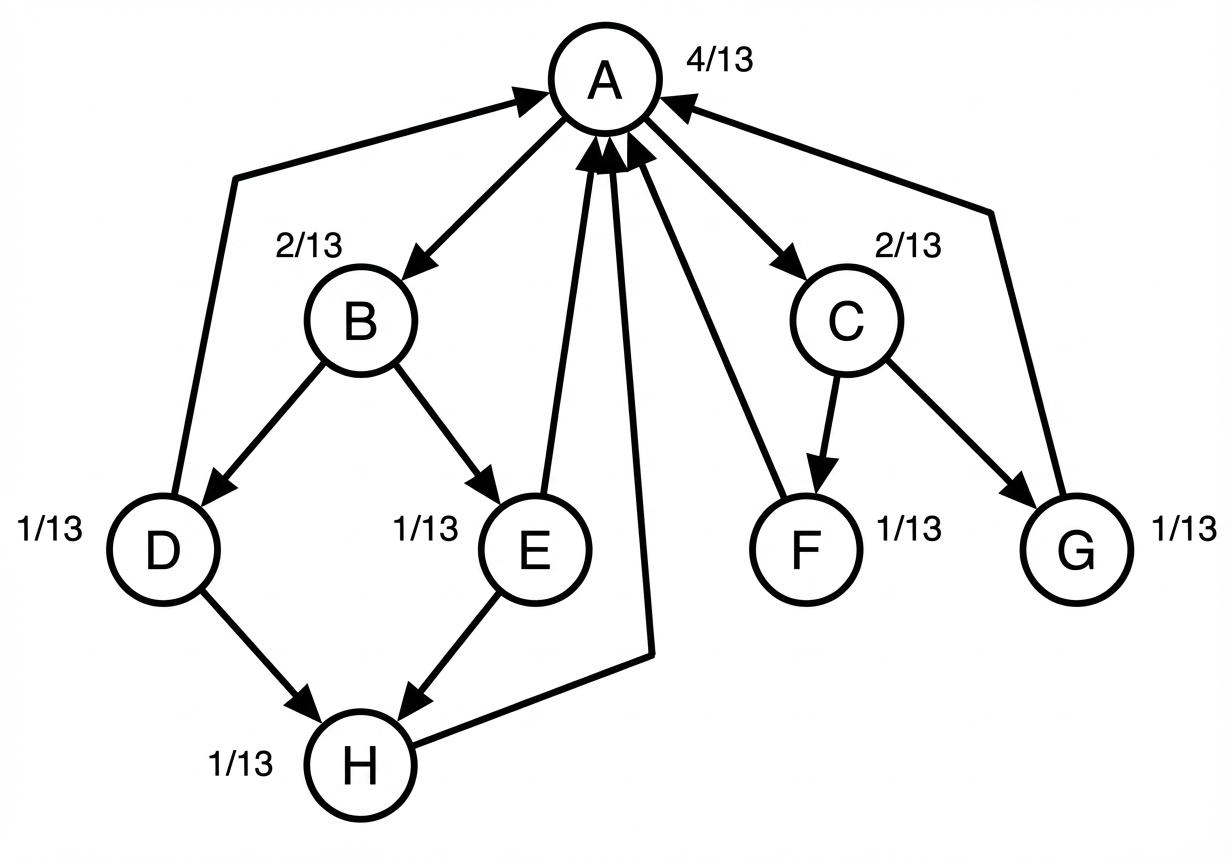
\includegraphics[width=0.6\linewidth]{images/WS_PR1.png}
    \caption{Vettore limite a partire da $f^{(0)}_i = \frac{1}{8}$}
    \label{fig:WS_PR1}
\end{figure}

Tuttavia, l'applicazione diretta di questo modello fallisce poiché il grafo del Web non è fortemente connesso. Come evidenziato nella \autoref{fig:WS_PR2}, ciò causa un accumulo irreversibile di fluido nelle componenti sconnesse (o "trappole"), dalle quali il rank non può più defluire, impedendo il raggiungimento di un equilibrio corretto.

\begin{figure}[ht!]
    \centering
    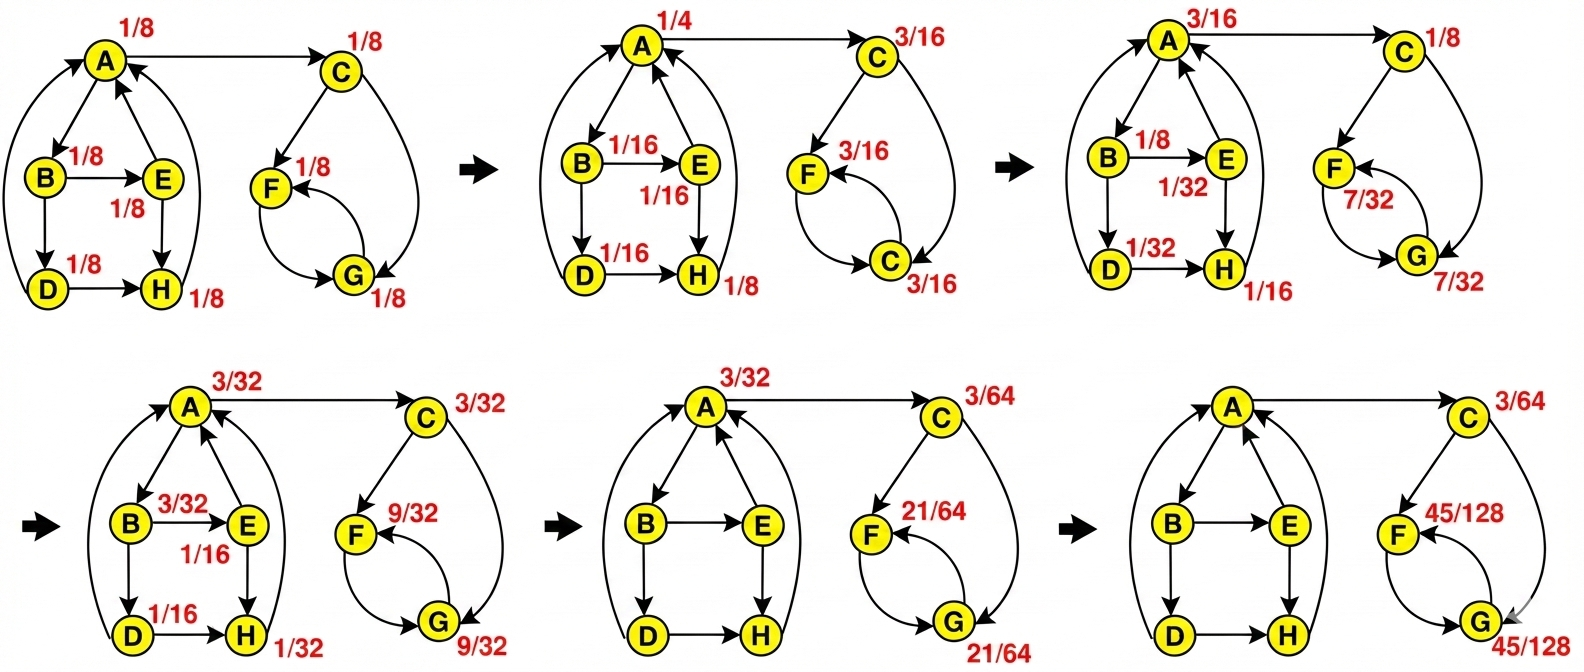
\includegraphics[width=0.8\linewidth]{images/WS_PR2.png}
    \caption{Contro esempio in cui il grafo è sconnesso}
    \label{fig:WS_PR2}
\end{figure}

\subsubsection{PageRank Scalato}

Come detto, se il grafo non è fortemente connesso (e il Web non lo è), il fluido (rank) si accumula nei nodi senza uscita e il resto della rete si svuota. er evitare questo blocco, si modifica il modo in cui il fluido viene distribuito ad ogni passo. Invece di passare tutto il rank ai vicini, se ne tiene una parte "di riserva" per ridistribuirla ovunque.

Viene introdotto un parametro $s \in [0,1]$ (chiamato solitamente \textit{damping factor}) che divide il rank di ogni nodo in due quote:

\begin{enumerate}
    \item La quota $s$: Una frazione pari a $s$ del rank del nodo viene distribuita equamente lungo gli archi uscenti (come nel PageRank classico).
    \item La quota $1 - s$: La parte rimanente, pari a $(1 - s)$, viene prelevata e distribuita uniformemente tra tutti i nodi del grafo (non solo ai vicini).
\end{enumerate}

Grazie a questa modifica, ad ogni iterazione ogni singolo nodo della rete riceve garantitamente una quantità minima di rank pari a:
\[
\frac{1 - s}{n}
\]

\begin{definizione}[Rank]
    Sia $r^{(k)}_i$ il rank posseduto dal nodo $i$ al passo $k$. Allora
    \[
    r^{(k+1)}_i = \left( \sum_{j=1: j \to i}^{n} r_j^{(k)}\frac{s}{\omega_j} \right) + \frac{1-s}{n}
    \]
\end{definizione}

Sia $N_{i,j}$ la matrice che descrive l'evoluzione del rank all'interno della rete, $\forall\ i,j = 1, \dots, n$.

\[
    N_{i,j} = 
    \begin{cases}
        \frac{s}{\omega_j} + \frac{1 - s}{n} \text{ if } j \to i \vspace{0.5 cm} \\ 
        \frac{1 - s}{n} \text{ otherwise}
    \end{cases}
\]

Infatti, sia $r^{(k)} = \left( r^{(k)}_1, r^{(k)}_2, \dots, r^{(k)}_n \right)$, l'elemento $i$-esimo di $N r^{(k)}$ è:

\begin{align*}
    \left(N r^{(k)}\right)_i = \sum_{j=1}^{n} N_{i,j} r_j^{(k)} 
    &= \sum_{j=1: j \to i}^{n} \left[ \frac{s}{\omega_j} + \frac{1 - s}{n} \right]r_j^{(k)} + \sum_{j=1: j \text{ non punta a } i}^{n} \frac{1-s}{n} r_j^{(k)} \\
    &= \sum_{j=1: j \to i}^{n} \frac{s}{\omega_j}r_j^{(k)} + \sum_{j=1}^{n} \frac{1-s}{n} r_j^{(k)} \\
    &= \sum_{j=1: j \to i}^{n} \frac{s}{\omega_j}r_j^{(k)} + \frac{1-s}{n} \underbrace{\sum_{j=1}^{n} r_j^{(k)}}_{= 1} \\
    &= \left(\sum_{j=1: j \to i}^{n} \frac{s}{\omega_j}r_j^{(k)}\right) + \frac{1-s}{n}
\end{align*}

Quindi, $r^{(k + 1)} = N r^{(k)}$. Analogamente al caso non scalato, possiamo pensare al vettore limite degli $r^{(k)}$, detto $r^*$, come ad un vettore che esprme una sorta di \textbf{configurazione di equilibrio} del rank, ossia redistribuendo il rank a partire da $r^*$, il vettore non varia: 
\[
r^* = N r^*
\]

Formalmente, il vettore limite desiderato deve corrispondere a un \textbf{autovettore stocastico} della matrice $N$, associato all'autovalore $\lambda=1$, con componenti non negative e somma pari a 1.
Il problema teorico fondamentale è dunque garantire che, per una generica matrice del Web, un tale autovettore \textbf{esista} e sia \textbf{unico}, assicurando così la stabilità del ranking.

Per dimostrare che questo autovalore esista, faremo utilizzo dei segeunti teoremi.

\begin{teorema}[Teorema di Perron]\label{teo:th_perron}
Sia $A$ una matrice reale quadrata $n \times n$ con elementi strettamente positivi. Allora valgono le seguenti proprietà:
\begin{enumerate}
    \item \textbf{Dominanza Spettrale:} La matrice $A$ possiede un autovalore reale positivo $c \in \mathbb{R}_{>0}$ che è strettamente maggiore in modulo di qualsiasi altro autovalore $\lambda$ della matrice (ovvero $c > |\lambda|$).
    \item \textbf{Autovettore Positivo e Unico:} Esiste un \textit{unico} autovettore $x$ associato a $c$ che soddisfa contemporaneamente le seguenti condizioni:
    \begin{itemize}
        \item Tutte le sue componenti sono reali e strettamente positive.
        \item La somma delle componenti è pari a 1 (normalizzazione).
    \end{itemize}
\end{enumerate}
\end{teorema}

\begin{definizione}[Matrice Stocastica]
Una matrice quadrata $A \in \mathbb{R}^{n \times n}$ si definisce \textbf{stocastica} se tutti i suoi elementi sono non negativi ($a_{ij} \ge 0$) e soddisfa una delle seguenti condizioni di normalizzazione:

\begin{itemize}
    \item \textbf{Stocastica per righe:} La somma degli elementi di ciascuna riga è uguale a 1.
    \[ \sum_{j=1}^n a_{ij} = 1 \quad \forall i \]
    \item \textbf{Stocastica per colonne:} La somma degli elementi di ciascuna colonna è uguale a 1.
    \[ \sum_{i=1}^n a_{ij} = 1 \quad \forall j \]
\end{itemize}
\end{definizione}

\begin{teorema}[Proprietà Spettrale delle Matrici Stocastiche]
Sia $A$ una matrice stocastica. Allora:

\begin{itemize}
    \item La matrice $A$ ammette sempre un autovalore $\lambda$ con modulo unitario ($|\lambda|=1$).
    \item Tale autovalore è dominante in modulo: per qualsiasi altro autovalore $\lambda'$ di $A$, vale la relazione $|\lambda'| \le 1$.
\end{itemize}
\end{teorema}

Poiché la matrice $N$ è costituita da elementi strettamente positivi, essa soddisfa pienamente le ipotesi del \autoref{teo:th_perron}.
Ciò ci garantisce che:
\begin{enumerate}
    \item Esiste un autovalore dominante $c$ reale e positivo.
    \item A tale autovalore corrisponde un autovettore $x$ \textbf{unico}, avente componenti tutte reali e positive, la cui somma è normalizzata a 1.
\end{enumerate}

Inoltre, dimostriamo che $N$ è una matrice \textbf{stocastica per colonne}. Infatti, sommando gli elementi di una generica colonna $j$, abbiamo che per ogni riga $i$:

\begin{proof}
    Poiché
    \[
        \sum_{i=1: j \to i}^{n} \frac{1}{\omega_j} = 1
    \]
    allora,
    \begin{align*}
        \sum_{i=1}^{n} N_{i,j} 
        &= \sum_{i=1: j \to i}^{n} \left[ \frac{s}{\omega_j} + \frac{1 - s}{n} \right] + \sum_{i=1: j \text{ non punta a } i}^{n} \frac{1-s}{n}\\
        &= \sum_{i=1: j \to i}^{n} \frac{s}{\omega_j} + \sum_{i=1}^{n} \frac{1-s}{n} = s + n \frac{1-s}{n} = 1
    \end{align*}
\end{proof}

\textbf{In conclusione}, $r^* = N r^*$.

\subsection{PageRank e RandomWalk}

Oltre all'interpretazione basata sul "fluido", il PageRank possiede una lettura probabilistica legata al concetto di \textit{random walk} (passeggiata aleatoria) su un grafo diretto $G = (V, A)$.

Immaginiamo un navigatore che si muove nella rete seguendo queste regole:
\begin{enumerate}
    \item \textbf{Inizializzazione:} Sceglie uniformemente a caso un nodo iniziale $u \in V$.
    \item \textbf{Navigazione:} Da $u$, sceglie uniformemente a caso un arco uscente che conduce a un nuovo nodo.
    \item \textbf{Iterazione:} Ripete il processo dal nuovo nodo, generando un percorso aleatorio infinito.
\end{enumerate}

Per analizzare la relazione tra questo processo e il PageRank, definiamo per ogni nodo $i \in V$ la variabile aleatoria $w_i^k$:
\[
w_i^k = 
\begin{cases} 
1 & \text{se al passo } k \text{ del random walk ci troviamo nel nodo } i \\
0 & \text{altrimenti}
\end{cases}
\]

Indichiamo con $f_i^{(k)}$ la probabilità di trovarsi nel nodo $i$ al passo $k$:
\[ f_i^{(k)} = \Pr\left[w_i^k = 1\right] \]

Il calcolo delle probabilità avviene induttivamente:

\begin{itemize}
    \item \textbf{Passo Base ($k=0$):} Poiché il nodo iniziale è scelto uniformemente tra gli $n$ nodi del grafo, la probabilità iniziale è:
    \[
    f_i^{(0)} = \Pr \left[w_i^0 = 1\right] = \frac{1}{n}
    \]
    
    \item \textbf{Passo Induttivo ($k > 0$):} Sia $\omega_j$ il numero di archi uscenti dal nodo $j$ (grado uscente). La probabilità di trovarsi in $i$ al passo $k$ dipende dalla probabilità di trovarsi in un nodo $j$ che punta a $i$ al passo precedente ($k-1$), moltiplicata per la probabilità di transizione $1/\omega_j$:
    \[
    f_i^{(k)} = \Pr\left[w_i^k = 1\right] = \sum_{j \in V : (j,i) \in A} \frac{1}{\omega_j} \Pr\left[w_j^{k-1} = 1\right] = \sum_{j \in V : (j,i) \in A} \frac{f_j^{(k-1)}}{\omega_j}
    \]
\end{itemize}

Nel modello scalato, introduciamo un parametro $s \in [0,1]$. Ad ogni passo il navigatore:
\begin{itemize}
    \item Con probabilità $s$ segue un arco uscente.
    \item Con probabilità $(1-s)$ salta uniformemente verso un qualsiasi nodo del grafo (teletrasporto).
\end{itemize}

Indichiamo con $sw_i^k$ la variabile aleatoria nel modello scalato. La relazione di ricorrenza diventa:

\[
\Pr\left[sw_i^k = 1\right] = \underbrace{\sum_{j \in V: (j,i) \in A} \frac{s}{\omega_j} \Pr\left[sw_j^{k-1} = 1\right]}_{\text{Navigazione Link}} + \underbrace{\frac{1-s}{n}}_{\text{Teletrasporto}} = r_i^{(k)}
\]

In questa ottica, il PageRank di una pagina rappresenta la probabilità stazionaria che un "navigatore casuale" si trovi su quella pagina dopo un numero sufficientemente grande di passi.